\cotefile{136}
\scanpage{235}

On considère l'anneau ½simplicial

\[
 \widehat A_*^*(S,\gamma^*,t)\deleted{\unsure{=|\mathrm{dfn}}}=\widehat A_*^*
\]

par

\[
\begin{aligned}
\widehat A_n^* &\simeq S\{\!\{X_0,\ldots,X_n\}\!\}\big/\bigl(\text{idéal \inserted{à p.d.,} \deleted{\unsure{fermé engendré}} engendré par }\textstyle\sum X_i-T\bigr)
 \otimes_S\frac{(\bigwedge^*[dX_0,\ldots,dX_n)}{\text{idéal }(\sum dX_i)}\\
 &(\simeq S\{\!\{Y_0,\ldots,Y_{n\unsure{-1}}\}\!\}[dY_0,\ldots,dY_{n-1}]
\end{aligned}
\]

On a donc \deleted{$\simeq$}

\[
 \widehat A_*^*\simeq\widehat A_*^0\otimes_S\bigwedge^*\Psi_*^S
\]

d'où

\[
 \pi_\ell(\widehat A_*^i)=\pi_\ell(\widehat A_*^0\otimes\bigwedge^i\Psi_*^S)\simeq\pi_{\ell-i}(\widehat A_*^0)
\]

et il faut donc étudier $\pi_*(\widehat A_*^0)$.

On considère sur $\widehat A_*^0$ \deleted{$\unsure{\Gamma_S^*(\Phi_*)}$} la filtration décroissante par idéaux fermés stables par p.d. ``engendrée'' par la condition que \deleted{\unsure{pour}} pour \unsure{tt|tout} $n$, les $X_i$ et $t$ soient en filtration $\geq 1$. On

\[
\begin{aligned}
\operatorname{Fil}^0(\widehat A_n^0)&\simeq \deleted{\unsure{S}}\widehat A_n^0\\
\operatorname{Fil}^p(\widehat A_n^0)&\simeq\left\{\sum\deleted{\unsure{a}}a_{i_0\ldots i_n}\deleted{\unsure{\{}}X_0^{(i_0)}\ldots X_n^{(i_n)}\ \middle|\ a_{i_0\ldots i_{\unsure{p|n}}}\in S^{[p-\sum_0^n i_\alpha]}\right\}\\
 &=\left\{\sum a_{i_0,\ldots i_{n-1}}Y_0^{(i_0)}\ldots Y_{n-1}^{(i_{n-1})}\ \middle|\ a_{i_0\ldots i_{\unsure{p|n|n-1}}}\in S^{p-\sum_0^n i_\alpha}\right\}
\end{aligned}
\]

Bien sûr, la topologie \unsure{produit|qui provient de} sur $\widehat A_n^{\unsure{*,0|*}}$ est aussi celle définie par cette filtration, et par suite $\widehat A_n^0$ est séparé et complet pour cette filtration. Un calcul immédiat donne, posant

\[
 k=S/S^{[1]}
\]

\[
 \operatorname{Gr}^{\unsure{p|1}}(\widehat A_*^0)
 \inserted{\simeq\widehat A_*^{p0}(\underbrace{\operatorname{Gr}^*(S),\widetilde\gamma^*,\widetilde t}_{\substack{k\text{-PD-algèbre}\\\text{\uline{graduée}}\\\text{quotient de }k\{T\}}})}
 \simeq\Gamma_k^p(\underline\Phi_*^k)
\]

\inserted{si l'épi $k\{T\}\longrightarrow\operatorname{Gr}^*(S)$ est un \uuline{iso}} \deleted{\unsure{d'où}}

d'où, dans cette hypothèse \inserted{d'isomorphisme}

\[
 \pi_i(\operatorname{Gr}^p(\widehat A_*^0))=
 \begin{cases}0&\text{si }p\ne0,\ i\ne0\ \deleted{\unsure{ou}}\\
 k&\text{si }(i,p)=0
 \end{cases}
 \quad(\text{donc }\operatorname{Gr}^p(\widehat A_*^0)\text{ flasque si }p\ne0)
\]

d'où on conclut que \deleted{l'inclusion}

\[
 \deleted{\operatorname{Fil}^1\widehat A_*^0\subset\widehat A_*^0}
\]

% archive sheet number: 234
\scanpage{236}

\mspage{- 188 -}

IX

\[
 \underline R_U/\underline R_U^f \simeq M_U \ , \tag*{(13.5.12)}
\]

et l'homomorphisme $i$ de (13.3.4) peut s'écrire comme un homomorphisme

\[
 i:M_U\longrightarrow A^{\handwritten{\natural}}\ , \tag*{(13.5.13)}
\]

qu'on retrouvera dans un contexte un peu différent au par. suivant.

14. \uline{Liens avec la théorie transcendante} : \uline{cas rigide-analytique}. \uline{L'homomorphisme canonique} $\underline M_K\longrightarrow A_K^{\handwritten{\natural}\unsure{o|0}}$.

14.1. Nous supposons connu ici les fondements de la théorie des espaces rigide analytiques, pour lesquels on pourra consulter [12] [13] [34].

Soit $S$ un trait complet, $A_K$ un schéma abélien sur son corps des fractions. On a construit alors dans 8.1, par descente à partir de l'extension de Raynaud dans le cas semi-stable, une extension $G_K=A_K^{\handwritten{\natural}o}$ (8.1.1)

\[
 0\longrightarrow T_K\longrightarrow G_K\longrightarrow B_K\longrightarrow0 \tag*{(14.1.1)}
\]

d'un schéma abélien $B_K$ par un tore $T_K$. Considérant le schéma abélien dual $A'_K$, on a de même une extension $G'_K=A_K^{\prime\handwritten{\natural}o}$

\[
 0\longrightarrow T'_K\longrightarrow G'_K\longrightarrow B'_K\longrightarrow0\ , \tag*{(14.1.2)}
\]

où $B'_K$ s'identifie d'ailleurs au schéma abélien dual de $B_K$ (8.2). On désigne, comme dans (8.1.8), par $\underline M_K$ et $\underline M'_K$ les réseaux sur $K$ duals de $T'_K$ et de $T_K$ respectivement :

\[
 \underline M_K=D(T'_K)\ ,\quad\underline M'_K=D(T_K)\ . \tag*{(14.1.3)}
\]

\handwritten{\unsure{506}}

\mspage{506}

% archive sheet number: 235
\scanpage{237}

\deleted{On trouve donc
\[
 H^i(C_{\mathrm{DR}}^*(X,\widehat A_*^*))=
 \begin{cases}H^0(X;S)&\text{si }i=0\\H^i(X,S^+)&\text{si }i\ne0\end{cases}
\]}

\[
\deleted{\unsure{E|\&}}\quad
\begin{cases}
 \operatorname{Fil}^p(\widehat A_*^0)\ \text{flasque pour tt }p\geq1\\
 \pi_i(\widehat A_*^0)=\begin{cases}0&\text{si }i\ne0\\ k&\text{si }i=0\end{cases}
 \quad\text{si }p\leq0
\end{cases}
\]

Considérons la filtration d'algèbre \inserted{½simpl.} sur $\widehat A_*^*$ prolongeant celle de $\widehat A_*^0$ et donnant \deleted{\unsure{aux}} à $\widehat A_*^1$ la filtration 1, donc

\[
 \operatorname{Fil}^p A_*^{*}=\sum_{0\leq i\leq p}\operatorname{Fil}^{p-i}(\widehat A_*^0)\otimes_S\bigwedge^i\deleted{\unsure{\underline\Phi}} \Psi_*
\]

\uline{C'est stable par l'opérateur différentiel}. On a \deleted{\unsure{donc}}

\[
\begin{aligned}
\pi_\ell(\operatorname{Fil}^p(A_*^i))
 &=\deleted{\sum_{0\leq\unsure{j|i}\leq p}}\pi_\ell(\operatorname{Fil}^{p-i}(\widehat A_*^0)\otimes_S\bigwedge^i\Psi_*)\\
 &\hspace{2em}\deleted{\pi_{\ell-i}(\operatorname{Fil}^{p-i}(\widehat A_*^0))}\\
 &=\pi_{\ell-i}(\operatorname{Fil}^{p-i}(\widehat A_*^0))\\
 &\quad\deleted{0\ \text{\unsure{sauf} si }\ell-i=\unsure{p-i}}\quad\deleted{\text{\unsure{i.e.} }\ell=p}\\
 &=\begin{cases}0&\text{si }\deleted{\ell\ne p}\ \text{ou }\unsure{i<p}\ \deleted{\unsure{\ell=p|\ell\ne p}}\deleted{\unsure{p\geq p}}\\[-2pt]
 &\inserted{p\leq i,\ \text{et }\ell=i}\ \deleted{\unsure{\text{et }p\leq}}\\
 k&\text{si }\deleted{\ell=p,\ i=p}\ p\leq i=\ell\end{cases}
\end{aligned}
\]

Donc \deleted{on en conclut la suite spectrale (pour $p$ fixé)} si on regarde $\operatorname{Fil}^p(A_*^*)$ comme \deleted{$E_2^{rs}=H^r(\unsure{\mathcal H}^s(X,\unsure{\mathcal F}$} une résolution ½simpliciale de $\deleted{\unsure{A}}S_*^{[p]}=\operatorname{Fil}^p S$, on voit que tous les termes $\operatorname{Fil}^p(A_*^i)$ de cette résolution \inserted{en degré $<p$} sont flasques, \deleted{\unsure{sauf}} après on a \deleted{\unsure{puis}}\deleted{\unsure{le premier}} $(j\geq p)$ $\operatorname{Fil}^p(A_*^j)\simeq\widehat A_*^0\otimes_S\bigwedge^j\Psi_*$ dont le seul groupe d'homotopie non nul est $\pi_j(\cdot)\simeq k$. On en conclut

\diagram{\begin{tikzcd}[ampersand replacement=\&,column sep=small]
 H^i\bigl(\underbrace{\operatorname{Fil}^p C_{\mathrm{DR}}^*(X,\widehat A_*^*)}_{\substack{\text{\unsure{2\textsuperscript{e} défn|cf. défn|$\simeq$ défn}}\\(C_{\mathrm{DR}}^*(X,\operatorname{Fil}\widehat A_*^*))}}\bigr)
 \arrow[r,"\sim"]\arrow[d] \& H^i(X,\underbrace{S^{[p]}}_{=\operatorname{Fil}^p S})\arrow[d]\quad\text{si }i\leq p\\
 H^i_{\unsure{1}}(C_{\mathrm{DR}}^*(X,\widehat A_*^*)\arrow[r] \& H^i(X,S)
\end{tikzcd}}

% archive sheet number: 236
\scanpage{238}

\mspage{- 186 -}

IX

\[
 {}_n A^{\unsure{o|0}}\simeq\underline R\otimes_{\mathbb Z}\mathbb Z/n\mathbb Z\ , \tag*{(13.5.5)}
\]

qui donne, pour $n$ parcourant les puissances d'un nombre premier $\ell$ donné, un isomorphisme de systèmes projectifs de groupes sur $S$

\[
 T_\ell(A^o)\simeq\underline R\otimes_{\mathbb Z}\mathbb Z_\ell\ , \tag*{(13.5.6)}
\]

où $\mathbb Z_\ell$ est considéré comme le système projectif des $\mathbb Z/\ell^{n+1}\mathbb Z$. Dans le cas envisagé ici où $A$ provient d'un schéma en groupes séparé sur $S$, on voit alors immédiatement que les $\underline R\otimes\mathbb Z/n\mathbb Z$ peuvent être considérés comme des schémas relatifs, ce qui donne un sens au symbole $(\underline R\otimes_{\mathbb Z}\mathbb Z_\ell)_{\underline O}$ (alors que $R_{\underline O}$ n'en aurait pas en général !), et on obtient un isomorphisme canonique

\[
 T_\ell(A_{\underline O})\overset{\handwritten{\unsure{!|1|\prime}}}{\simeq}(\underline R\otimes_{\mathbb Z}\mathbb Z_\ell)_{\underline O}\ . \tag*{(13.5.7)}
\]

Il résulte alors immédiatement des constructions du par. 2 et de 13.3 que l'isomorphisme précédent transforme partie fixe en partie fixe, partie torique en partie torique :

\[
 T_\ell(A_{\underline O})^f\simeq(\underline R^f\otimes_{\mathbb Z}\mathbb Z_\ell)_{\underline O}\ ,\quad T_\ell(A_{\underline O})^t\simeq(\underline R^t\otimes_{\mathbb Z}\mathbb Z_\ell)_{\underline O}\ . \tag*{(13.5.8)}
\]

Si $A'$ est un groupe analytique relatif sur $S$ satisfaisant aux mêmes hypothèses que $A$, et si $W_{\underline O}$ est une biextension de $(A_{\underline O},A'_{\underline O})$ par $\mathbb G_{m\underline O}$, définissant donc au-dessus d'un voisinage de $s$ une biextension de $(A,A')$ par $\mathbb G_{mS}$ (en travaillant maintenant avec la notion au sens analytique complexe, obtenue en travaillant dans le site des espaces analytiques au-dessus de $S$, pour une topologie convenable \ldots), alors d'après VIII 2.2 $W$ définit des accouplements

\handwritten{504}

\mspage{504}

% archive sheet number: 237
\scanpage{239}

qui s'écrit aussi

\diagram{\begin{tikzcd}[ampersand replacement=\&,column sep=small]
 H^i(\operatorname{Fil}^p C^*_{\mathrm{DR}}(X;S,t,\gamma^*))\arrow[r,"\sim"]\arrow[d]
 \& H^i(X,\operatorname{Fil}^p S)\arrow[d]\quad\substack{\text{\tikz[baseline=(w.base)]\node[draw,ellipse,inner sep=1pt](w){\uuline{iso si}};}\\\text{\uuline{$i\leq p$}}}\\
 q\leq p\quad H^i(\operatorname{Fil}^q C^*_{\mathrm{DR}}(X;S,t,\gamma^{\prime}))\arrow[r]
 \& H^i(X,\operatorname{Fil}^q S\quad\substack{\text{\uuline{iso} si}\\i\leq q}
\end{tikzcd}}

\uline{NB} Si on ne suppose pas que l'épi

\[
 k\{T\}\unsure{\relbar|\longrightarrow}\operatorname{Gr}^*(S)
\]

est un iso, on ne peut rien dire. Prenons p.ex. le cas extrême de dégénérescence

\[
 t=0,\quad\text{donc}\quad S\xrightarrow{\sim}k
\]

on a alors

\[
 \operatorname{Gr}^p\widehat A_*^{\deleted{\unsure{*}}0}\simeq\Gamma_k^p(\Psi_*)\ ,
\]

donc

\[
 \operatorname{Gr}^p(\widehat A_*^{\deleted{\unsure{*}}0})\simeq\Pi_*(k,p)
\]

qui n'est flasque pour aucun $p\geq0$ (si $k\ne0$).

Prenons aussi le cas de $(\mathbb Z_p,p)$, la pd-filtration définie par $p$ est cofinale à la filtration $p$-adique si $p\ne2$ (si $p=2$, c'est la filtration constante de valeur $\operatorname{Fil}^{\unsure{p|r}}\mathbb Z_2=2\mathbb Z_2$ si $p\geq1$, donc $\operatorname{Gr}^*(S)\simeq\operatorname{Gr}^{0}_{\unsure{0}}(S)\simeq\mathbb F_2$ dans ce cas, i.e. c'est \unsure{encore} le cas de dégénérescence\ldots.), quel est exactement l'idéal \deleted{$S^{[i]}=(\frac{p^{n'}}{n!}\mathbb Z_p)=$ i.e. quelle} $S^{[i]}$ engendré par les $\frac{p^{\unsure{j|i}}}{j!}$ pour $j\geq i$ ? \deleted{\unsure{i.e. quel est son|i.e. probablement}}

% archive sheet number: 238
\scanpage{240}

\mspage{- 185 -}

IX

phisme (i.e. tel que $\underline O_S\longrightarrow f_*(\underline O_{S'})$ soit injectif) est un \uline{morphisme de descente effective} pour la catégorie fibrée des schémas abéliens relatifs.

b) Il semble que la méthode de démonstration de 13.5.2 doive permettre aussi de prouver le résultat analogue pour tout espace analytique $B$ propre sur $S$. Plus délicate sans doute est la question de savoir si, pour un espace analytique $X$ propre sur $S$, tel que le complété formel $\widehat X$ le long de $X_s$ soit algébrisable, $X$ est algébrisable sur $S$ au voisinage de $s$. Signalons seulement qu'il y a lieu ici de prendre la notion d'algébrisabilité relative de $X$ sur $S$ dans un sens plus large que dans [10], en entendant par là qu'au voisinage de $s$, $X$ provient d'un \uline{espace algébrique} sur $\underline O_{S,s}$ au sens de M. ARTIN [1].

13.5.4. Plaçons-nous dans les conditions de 13.5.1. Choisissons par ailleurs, pour tout entiers $n>0$, l'isomorphisme standart de groupes sur $\mathbb C$

\[
 \handwritten{\mu}_{n\mathbb C}\simeq(\mathbb Z/n\mathbb Z)_C\ ,\quad m\longmapsto\exp(2i\pi m/n)\ ,
\]

ce qui nous donne, par passage à la limite sur les puissances d'un nombre fixé $\ell$, un isomorphisme canonique de faisceaux $\ell$-adiques sur $\mathbb C$ :

\[
 \mathbb Z_\ell(1)_{\mathbb C}\simeq\mathbb Z_{\ell\mathbb C}\ ,
\]

que nous utiliserons pour identifier les deux membres.

De la suite exacte (13.1.3), on déduit, en appliquant la suite exacte des $\underline{\operatorname{Ext}}_{\mathbb Z}^i(\mathbb Z/n\mathbb Z,-)$, un isomorphisme canonique

\handwritten{503}

\mspage{503}

% archive sheet number: 239
\scanpage{241}

\[
 v_p(n!)=\frac{1}{p-1}(n-\operatorname{chiff}_p n)
\]

\[
 v_p(p^{(n)})=v_p\left(\frac{p^n}{n!}\right)=\frac{1}{p-1}\bigl((p-2)n+\underline{\operatorname{chiff}_p n}\bigr)
 \quad(=\operatorname{chiff}_p(n)\ \text{si }p=2)
\]

\deleted{Si $p$}

\[
\begin{aligned}
 \gamma_{p,i}&=\mathop{\mathrm{Inf}}_{\underline n\geq i.}v_p(p^{(n)})
 =\mathop{\mathrm{Inf}}_{\underline n\geq i}\frac1{p-1}\bigl(\underbrace{(p-2)n+\operatorname{chiff}_p(n)}_{\substack{\text{cette fonction en }n\\\text{n'est ni croissante}\\\text{ni décroissante\ldots.}}}\bigr)\\
 &=\begin{cases}1&\text{si }p=2\\
 >\dfrac{p-2}{p-1}i\xrightarrow[i\to+\infty]{}+\infty&\text{si }p\ne2\end{cases}
\end{aligned}
\]

\[
 i=i_0+i_1p+\ldots+i_{\unsure{r|v}}p^r
\]

\deleted{\unsure{Si i|Si|donc}} \deleted{$i_0$} \deleted{$\unsure{i_0|\text{si}}$}

\[
 \underbrace{\underbrace{(p-1)}_{i_0}+\ldots+\underbrace{(p-1)}_{i_{s-1}}p^{s-1}}_{p^{\unsure{s+1|s}}-1}
 +\underset{\substack{\wedge\\p-1}}{i_{s\deleted{\unsure{+1}}}}p^{s\deleted{\unsure{+1}}}\ldots+i_r p^r
\]

\[
 i+1=i_{s\deleted{\unsure{+1}}}p^{s\deleted{\unsure{+1}}}+\ldots+i_rp^r
\]

\[
 (p-2)i+(p-1)s\deleted{\unsure{+1}}+\deleted{\sum_{\alpha\geq s}i_\alpha}
 \leq(p-2)(i+1)+\deleted{\sum_{\alpha\geq s}i_{\alpha\unsure{\prime}}}
\]

\[
\begin{aligned}
 [v_p(p^{(i)})\leq v_p(p^{(i+1)})]&\unsure{\Leftrightarrow|\Rightarrow}
 [(p-1)s\leq(p-2)]\Longleftrightarrow[s=0]\Longleftrightarrow[i_0\ne p-1]\\
 &\deleted{\boxed{i_0<p-1}}\Longleftrightarrow i+1\not\equiv0\ (p)
\end{aligned}
\]

Exemple où $\gamma_{p,i}=\gamma_{p,i+1}$ : Il \uline{suffit} qu'on ait \deleted{$v_p(\unsure{p^{i}}$}

\[
 v_p(p^{(i+1)})\leq v_p(p^{(i)})
\]

i.e. que \deleted{dans la \unsure{base}}\quad\deleted{\unsure{pour la der}} $i+1\equiv0\ (p)$ i.e. $i$ de la forme $p\unsure{l|\ell}-1$

% archive sheet number: 240
\scanpage{242}

\mspage{- 182 -}

IX

13.5. \uline{Cas d'une situation relativement algébrique}. Nous supposons maintenant que $A$ provient d'un schéma en groupes relatif sur $S$, lisse, séparé et à fibres des extensions de schémas abéliens par des tores.
% Short mark just below "par", adjoining a vertical trace.

Nous désignerons ce schéma relatif par la même lettre $A$. (Nous nous autorisons cet abus de notation grâce au fait que le foncteur $G\mapsto G^{\mathrm{an}}$, qui va de la catégorie des schémas en groupes relatifs du type envisagé vers la catégorie des groupes analytiques sur $S$, est pleinement fidèle, comme il serait facile à établir grâce aux résultats du type GAGA relatifs [10].) Pour tout ce qui concerne la notion de schéma re\uuline{la}tif, et les relations entre schémas relatifs sur $S$ et espaces analytiques sur $S$, nous renvoyons à [10] (cf. aussi [2, Exp. 15]). Si $\underline O$ désigne l'anneau local de $S$ en $s$, le schéma relatif $A$ est connu au voisinage de $s$ par la connaissance du schéma ordinaire $A_{\underline O}$ sur $\operatorname{Spec}(\underline O)$, déduit de $A$ par localisation en $s$. Il est clair alors que le complété formel de $A_{\underline O}$ le long de sa fibre spéciale (isomorphe à $A_s=A_{\unsure{o|0}}$) est isomorphe au complété formel du groupe analytique $A$ le long de $A_s$ (13.2), en identifiant les $A_n=A\times_S S_n$ à des schémas algébriques sur $S$, par l'abus de notations introduit ci-dessus. Dans le cas favorable où $\widehat A$, regardé comme schéma formel en groupes sur $\widehat{\underline O}$, est algébrisable (7.2.1), ce qui est le cas en particulier si $S$ est normal en $s$ et $A$ quasi-projectif sur $S$ (7.1.5) on obtient donc un schéma en groupes $A^{\handwritten{\natural}}_{\widehat{\underline O}}$ sur $\operatorname{Spec}(\widehat{\underline O})$, extension d'un schéma abélien $B_{\widehat{\underline O}}$ par un tore. Pour simplifier, nous supposons que $B_{\widehat{\underline O}}$ est projectif sur $\widehat{\underline O}$ (ce qui est bien le cas, on le sait, si $\underline O$ donc $\widehat{\underline O}$ est normal). On va alors prouver :

\handwritten{\unsure{1}}

\handwritten{500}

\mspage{500}

% archive sheet number: 241
\scanpage{244}

\margin{Généralités sur modules gradués sur certains anneaux gradués}

$S$ anneau $\mathbb Z$-gradué \unsure{disons|comm.} à degrés $\geq0$ \quad $S^0=k$

$\mathcal M$ catégorie des $S$-modules gradués

\textcircled{$T$} foncteur translation : $T(M)_{\unsure{i|n}}=M_{i+1}$ \inserted{(autom. de $\mathcal M$)}

$T^{\unsure{n|i}}$ itéré \unsure{i.ème|n.ème} ($i\in\mathbb Z$) \quad $T^i(M)_{\unsure{n|i}}=M_{\unsure{i+n|n+i}}$

$\tikz[baseline=(m.base)]\node[draw,ellipse,inner sep=1pt](m){$\mathcal M^+$};\subset\mathcal M\mid S$-modules gradués à degrés $\geq0$

N.B. $\boxed{T^{-1}(\mathcal M^+)\subset\mathcal M^+}$

\[
 T^{-{\deleted{\unsure{n}}N}}(\mathcal M^+)=\mathcal M_N^{\unsure{*}}
 \quad S\text{-modules gradués à degrés }\geq N
\]

\inserted{$(\deleted{\unsure{M}}\mathcal M_0=\mathcal M^+)$}

\[
 \mathcal M\qquad \deleted{\unsure{M}}N\leq N'\Longrightarrow\mathcal M_N\supset\mathcal M_{N'}
\]

$\mathcal N=$ catégorie des $k$-modules (pas gradués)

\[
 M_0\longrightarrow M_0\otimes_k S
\]

\tikz[baseline=(m.base)]\node[draw,ellipse,inner sep=0pt](m){$\boxed{\mathcal N\xrightarrow{\varphi}\mathcal M}$}; se factorise par $\mathcal M^+=\mathcal M_0$

\textcircled{1} Étude de l'inclusion (pl. fid.)

\[
 \mathcal M_{\deleted{\unsure{M}}N'}\lhook\joinrel\xrightarrow[i_{N,N'}]{}\mathcal M_N\qquad N'\geq N
\]

Commute aux $\underrightarrow{\lim}$ et $\underleftarrow{\lim}$, donc on s'attend à trouver des adjoints à g. et à dr.

\uline{Adjoint à droite} \inserted{$\tau_{N',N}$} \uline{de} $i_{N,N'}$

\[
 \tau_{N',N}:\mathcal M_N\longrightarrow\mathcal M_{N'}
\]

\[
 \tau_{N',N}(M)_i=\begin{cases}0&\text{si }i<N'\\M_i&\text{si }i\geq N'\end{cases}
\]

C'est un \uline{sous-module} de $M\in\operatorname{Ob}\mathcal M_N$ (car $S$ à degrés $\geq0$)

% printed form
% upside down
\deleted{5-856\\
M. GROTHENDIECK ALEXANDRE\\
PROFESSEUR\\
MATHEMATIQUES}

% archive sheet number: 243
\scanpage{245}

% letterhead
Le Professeur Pierre, Robert LAFON\\
Directeur de l'U.E.R. IX\\
de l'Université Paul Valéry\\
-{}-{}-{}-{}-{}-{}-{}-\\
LE QUEBEC ``C''\\
Avenue des Etats du Languedoc\\
34000 MONTPELLIER\\

Montpellier, le 20 mai 1975\\

à\\
Monsieur le Directeur\\
de l'U.E.R.\\
de l'Université\\
de Montpellier\\

Monsieur le Directeur et Cher Collègue,\\

Comme vous le savez, une \textit{Université du 3ème Age} a été créée dans l'U.E.R. IX de l'Université Paul Valéry.

Après trois mois d'expérience, il s'avère que cette création correspond à un besoin de la population, puisque plus de \textit{``500 étudiants''} fréquentent les diverses activités entreprises au cours de cette année expérimentale. Nous devons nous attendre à un effectif plus important à la prochaine rentrée universitaire, aussi, je serais désireux de multiplier les enseignements et je vous serais reconnaissant si vous pouviez demander aux Collègues de votre U.E.R., s'ils accepteraient éventuellement de participer à cet enseignement et de me faire des propositions, afin qu'en accord avec les étudiants du 3ème Age, nous puissions mettre sur pied le programme de l'année 75/76.

Ces enseignements peuvent être faits, sous forme de conférences magistrales isolées, d'heures de cours hebdomadaires ou mensuels, ou de sessions intensives. Il peut y avoir également des visites organisées ou des activités pratiques.

Sans doute, je pourrais faire appel au bénévolat, mais je pense qu'il est plus convenable d'honorer selon les règles de l'Education Nationale, les collègues qui accepteraient de participer à ces enseignements.

Je vous serais reconnaissant de diffuser cette lettre aux membres de votre U.E.R., en demandant à nos collègues une réponse assez rapide, soit par lettre, soit en prenant contact avec moi, directement à mon domicile, par téléphone, au 58.24.50, de préférence en début d'après midi.

Je vous remercie de l'aide que vous voudrez\\
bien m'apporter dans le développement de cette Université et vous prie de croire,\\
Monsieur le Directeur et cher Collègue, à l'expression de mes sentiments les plus\\
dévoués.\\

Diffusion : Liste B - n° 3211\\

\handwritten{\unsure{Lafon|P.R. Lafon}}\\

\figure{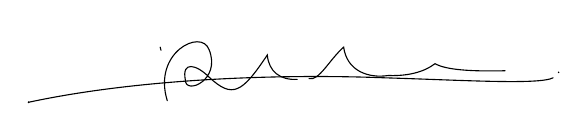
\begin{tikzpicture}[x=1cm,y=1cm,line cap=round]
\draw (0,0) .. controls (1.45,.31) and (3.25,.36) .. (4.53,.31) .. controls (5.53,.28) and (6.48,.22) .. (6.66,.31);
\draw (1.76,.02) .. controls (1.57,.63) and (2.19,.94) .. (2.29,.67) .. controls (2.45,.28) and (1.99,.09) .. (1.99,.28) .. controls (1.94,.53) and (2.13,.48) .. (2.29,.32) .. controls (2.59,.04) and (2.71,.12) .. (3.03,.60) .. controls (3.05,.39) and (3.19,.28) .. (3.41,.29);
\draw (3.56,.30) .. controls (3.69,.27) and (3.81,.53) .. (4,.70) .. controls (4.04,.40) and (4.31,.30) .. (4.57,.34) .. controls (4.80,.33) and (5.02,.38) .. (5.16,.49) .. controls (5.30,.41) and (5.62,.39) .. (6.05,.40);
\draw (1.68,.66)--(1.67,.70);
\fill (0,0) circle (.013); \fill (6.73,.38) circle (.011);
\end{tikzpicture}}

Transmis pour information\\
et suite à donner.\\

Les Directeurs d'U.E.R. d'Enseignement\\

Pr P.R. LAFON\\

% archive sheet number: 244
\scanpage{246}

\[
 \tau_{N',N}(M)\hookrightarrow M
\]

Soit $M\in\operatorname{Ob}\mathcal M_N$, $\deleted{\unsure{N}}P\in\operatorname{Ob}\mathcal M_{N'}$,

\diagram{\begin{tikzcd}[ampersand replacement=\&,column sep=small]
 \operatorname{Hom}_{\mathcal M_N}(i_{N,N'}(P),M)\arrow[d,equal]
 \& \operatorname{Hom}_{\mathcal M_{N'}}(P,\tau_{N',N}(M))\arrow[l,"\sim"']\arrow[d,equal]\\
 \operatorname{Hom}_{\mathcal M}(P,M)
 \& \operatorname{Hom}(P,\tau_{N',N}(M))\arrow[l,"\sim"']
\end{tikzcd}}

\uline{Adjoint à gauche} $q_{N',N}$ \uline{de} $i_{N,N'}$

\[
 \begin{aligned}
 \operatorname{Hom}_{\mathcal M_N}(M,i_{N,N'}(\deleted{\unsure{A}}P))&=\\[-2pt]
 \shortparallel\qquad &\\[-2pt]
 \operatorname{Hom}_{\mathcal M}(M,P)&=\operatorname{Hom}_{\mathcal M}(M/\substack{\text{ss-module}\\\text{engendré par}\\\text{les }M_i,\ i<N'},P
 \end{aligned}
\]

\diagram{\(\begin{array}{cccccccccc}
 0&0\,\cdot&M_N&M_{N+1}&M_{N+2}&\ldots&M_{N'-1}&M_{N'}&M_{N'+1}&\ldots\\
 &0&0&0&0&\ldots&0&\deleted{\unsure{M}}P_{N'}&\deleted{\unsure{M}}P_{N'+1}&\ldots
\end{array}\)}

\[
 q_{N',N}(M)=M/\substack{\text{ss-module de }M\text{ engendré}\\\text{par les }M_i,\ i<N'}
\]

\uline{NB} $q_{N',N}$ et $\tau_{N',N}$ sont des ``foncteurs de localisation'' (car adjoints d'un foncteur pl. fid.) ; \deleted{et} $q_{N',N}$ est exact à droite (en fait, \inserted{$q_{N',N},i_{N,N'},\tau_{N',N}$ commutent aux $\underrightarrow{\lim}$ quelc.}) mais en général pas à gauche sans doute -- on ne s'attend pas qu'il ait encore un adj. à g. Par contre $\tau_{N',N}$ commute aux $\underleftarrow{\lim}$ \uline{et} aux $\underrightarrow{\lim}$ (à fortiori il est exact). On s'attend à en trouver un foncteur adjoint à droite.

% archive sheet number: 245
\scanpage{247}

\deleted{\diagram{\resizebox{\linewidth}{!}{\begin{tikzcd}[ampersand replacement=\&,column sep=0.45em,row sep=0.5em]
 A^* \& \cdot\arrow[d,no head] \& d\arrow[d,no head]\& J\arrow[d,no head] \& \gamma\arrow[dd,no head,bend right=12]\quad\deleted{\unsure{\text{sous}|\text{puiss.}}}\\
 \substack{\circledast\ \text{groupe gradué}\\\text{à degrés }\geq0}\arrow[dr,no head]
 \& \substack{\circledast\ \text{multiplication}\\\text{associative}\\\text{unitaire}\\\deleted{\unsure{\text{sur }A^0}}}\arrow[d,no head]
 \& \substack{\circledast\ \text{différentielle}\\d^2=0\\\circledast\ d\text{ de degré }+1\\
 \circledast\ d(xy)=(dx)y\\{}+(-1)^{\deg x}x\,dy}
 \&[-.5em]\substack{\text{Sous-groupe}\\
 \circledast\ \text{contient } A^+=\sum_{i>0}A^i,\ \text{donc}\\
 \deleted{\text{gradué}}\ \inserted{\text{de la forme}}\\J^0+\sum_{i>0}A^i\\
 \circledast\ \text{idéal (i.e. }J^0\text{ idéal)}\\
 \circledast\ \text{stable par }d\text{ (automatique)}}\&\\
 \&\substack{\circledast\ \text{alg. graduée}\\x\in A^i,\ y\in A^j\Rightarrow xy\in A^{i+j}\\
 \text{alg. alternée, i.e.}\\
 \left\{\begin{smallmatrix}xy=(-1)^{ij}yx\\x^2=0\ \text{si }x\in A^i,\ i\text{ impair}\end{smallmatrix}\right.}
 \& \& \&\substack{\circledast\ \text{puissances divisées sur }J\\\deleted{x^{(\alpha)}=0}\\
 \circledast\ x\in A^i\Longrightarrow x^{(\alpha)}\in A^{\alpha i}\\
 \circledast\ \deleted{d(x^{\alpha})=}\quad x\in\sum_{i\ \mathrm{imp}}A^i,\ \deleted{i\ \mathrm{impair}},\ \alpha\geq2\\
 x,\in{}A^{\unsure{1|i}},y\in A\ \Rightarrow x^{(\alpha)}=0\\
 \circledast\ d\,x^{(\alpha)}=x^{(\alpha\unsure{+|-}1)}dx}
\end{tikzcd}}}}

\[
\begin{aligned}
 &\deleted{A^{\unsure{0|\oplus}}_+}\\
 &\deleted{A^{\mathrm{pair}}+A^{\mathrm{impair}}=A^0+A^1}\\
 &\deleted{J^0\ -}\\
 &\deleted{\left(\sum_{i\ \mathrm{pair}}x_i+\sum_{j\ \mathrm{impair}}x_j\right)^\alpha}
\end{aligned}
\]

\[
\begin{aligned}
 &\deleted{A^0+\underbrace{A^1}_{\deleted{\unsure{\text{idéal}}}}}\qquad
 \deleted{\left(\unsure{\sum_i} x_i\right)^{\unsure{p|2}}=\sum_i x_i x_j+}
 \qquad \deleted{\bigwedge^2 A^1\unsure{\longrightarrow|-}J^0\subset A^0}\\
 &\deleted{(x+y)^2=x^2+y^2+xy+yx}\\
 &\deleted{J^0+A^1=J}\qquad \deleted{A^0\cdot A^1\subset A^1,\quad A^1 A^1\subset A^0}
\end{aligned}
\]

\[
\begin{aligned}
 &\deleted{(\overset{\downarrow}{x}+\overset{\downarrow}{y})^{(\alpha)}
 =\deleted{\sum}x^{(\alpha)}+x^{(\alpha-1)}y+
 \deleted{x^{(\alpha-2)}y^{(2)}}\ \unsure{\ldots}\quad\deleted{(x+y)^\alpha}}\\
 &\deleted{z^{(\alpha)}=(\underline{x+y})^{(\alpha)}=x^{(\alpha)}+x^{(\alpha-1)}y}\\
 &\deleted{z'^{(\alpha)}=(x'+y')^{(\alpha)}=x'^{(\alpha)}+x'^{(\alpha-1)}y'}
\end{aligned}
\]

\[
\begin{aligned}
 &\deleted{(x+x')}\\
 &\deleted{(z+z')^{(\alpha)}=((x+x')+(y+y'))^{(\alpha)}=(x+x')^{(\alpha)}+(x+x')^{(\alpha-1)}(y+y')}\\
 &\deleted{\phantom{(z+z')^{(\alpha)}}=\sum_{i+j=\alpha}x^{(i)}x'^{(j)}
 +\left(\sum_{i+j=\alpha-1}x^{(i)}x'^{(j)}\right)(y+y')}\\
 &\deleted{\unsure{\shortparallel?}}
\end{aligned}
\]

\[
\begin{aligned}
 &\deleted{\sum_{i+j=\alpha}z^{(i)}z'^{(j)}=\sum_{i+j=\alpha}(\deleted{\unsure{z}}x^{(i)}+x^{(i-1)}y)(x'^{(j)}+x'^{(j-1)}y')}\\
 &\deleted{\qquad=\sum_{i+j=\alpha}x^{(i)}x'^{(j)}+\left(\sum_{i+j=\alpha-1}x^{(i)}x'^{(j)}\right)(y+y')}\\
 &\deleted{\qquad\quad+\left(\sum_{i+j=\alpha-2}x^{(i)}x'^{(j)}\right)yy'}\\
 &\deleted{\boxed{\text{OK si }yy'=0}}
\end{aligned}
\]

% archive sheet number: 246
\scanpage{248}

D'ailleurs $\deleted{\unsure{q}}\tau_{N',N}$, étant un foncteur de localisation exact, commut\deleted{\unsure{e}}ant aux $\underrightarrow{\lim}$, est un foncteur de passage au quotient modulo une ss-catégorie abélienne épaisse stable par $\underrightarrow{\lim}$ -- savoir la sous-catégorie des $M$ \deleted{\unsure{(}} tels que \deleted{$M_i$} ($\tau_{N',N}M=0$ i.e.) $M_i=0$ pour $i\geq N'$

\uline{Adjoint à droit} $\rho_{N,N'}$ \uline{de} $\tau_{N',N}$

\diagram{\begin{tikzcd}[ampersand replacement=\&,column sep=small,row sep=small]
 \operatorname{Hom}_{\mathcal M_{N'}}(\tau_{N',N}(M),P)\arrow[d,equal]\arrow[r,phantom,"{\overset{?}{\unsure{\simeq|\xrightarrow{\sim}}}}" description]
 \&\operatorname{Hom}_{\mathcal M_N}(M,\rho_{N,N'}P)\\
 \operatorname{Hom}_{\mathcal M}(\tau_{N',N}(M),P)\arrow[d,phantom,"\cap" description]\&\\
 \displaystyle\prod_{i\geq N'}\operatorname{Hom}_k(M_i,P_i)\&
\end{tikzcd}}

\diagram{\begin{tikzcd}[ampersand replacement=\&,column sep=.4em,row sep=.5em]
 0\&0\&M_N\&M_{N+1}\&\ldots\&M_{N'-1}\&M_{N'}\arrow[d]\&M_{N'+1}\arrow[d]\&\ldots\\
 0\&0\&0\&0\&\&0\&P_{N'}\&P_{N'+1}\&\ldots
\end{tikzcd}}

\[
\begin{aligned}
 &\deleted{\rho_{N,N'}(P)_i=\begin{cases}P_i&\text{\unsure{si} }i\geq N'\\
 \unsure{\subset}\ \text{si }i<N'\ \unsure{\subset}\displaystyle\prod_{\unsure{j\geq N'-i}}\operatorname{Hom}_{\unsure{k_0|k}}(S_j,P_{i+j})&\end{cases}}\\
 &\deleted{\qquad\operatorname{Hom}_{\mathcal M}(\underbrace{T^{-i}\tau_{N'-i,0}S}_{\in\mathcal M_{N'}},P)}\\
 &\deleted{\qquad=\operatorname{Hom}^i(\tau_{N'-i,0}(S),P)}
\end{aligned}
\]

\[
\begin{aligned}
 \rho_{N,N'}(P)_i&=\begin{cases}0&\text{si }i<N\deleted{\unsure{\prime}}\\
 \operatorname{Hom}_{\mathcal M}^i(\tau_{N'-i}S,P)&\end{cases}\\
 &\qquad\simeq\operatorname{Hom}_{\mathcal M_N}(T^{-i}\tau_{N'-i}S,P)\\
 &\hspace{8em}\text{si }i\geq N
\end{aligned}
\]

% archive sheet number: 247
\scanpage{249}

\diagram{\begin{tikzcd}[ampersand replacement=\&,column sep=.25em,row sep=.1em]
 (\lambda\&\cdot z)^{(\alpha)}\overset{?}{=}\lambda^\alpha z^{(\alpha)}\\
 A\arrow[u]\&J\arrow[u]
\end{tikzcd}}

\[
 \left(\sum_{i\,\mathrm{imp}}x_i\right)\left(\sum_{j\,\mathrm{imp}}y_j\right)=\sum_{i,j}x_i y_j
\]

\[
\begin{aligned}
 \lambda&=\underset{\substack{\uparrow\\A^0}}{\zeta}+\underset{\substack{\uparrow\\A^1}}{\eta}\qquad z=x+y\\
 \lambda z&=\deleted{\underset{\substack{\uparrow\\ A^0}}{(\zeta x+\eta y)}+(\zeta y+\underbrace{\eta x}_{x\eta})}
\end{aligned}
\]

\[
\begin{aligned}
 (\lambda z)^{(\alpha)}&=(\zeta x+\eta y)^{(\alpha)}+(\zeta x+\eta y)^{(\alpha-1)}(\zeta y+x\eta)\\
 &=\sum_{i+j=\alpha}(\zeta x)^{(i)}(\eta y)^{(j)}
 +\left(\sum_{i+j=\alpha-1}(\zeta x)^{(i)}(\eta y)^{(j)}\right)(\zeta y+x\eta)
\end{aligned}
\]

\deleted{\[
\begin{aligned}
 \lambda^\alpha z^{(\alpha)}&=(\zeta^\alpha+\alpha\zeta^{\alpha-1}\eta)(x^{(\alpha)}+x^{(\alpha-1)}y)\\
 &=(\zeta^\alpha x^{(\alpha)}+\alpha\zeta^{\deleted{\unsure{\alpha-1}}\alpha-1}x^{(\alpha-1)}\eta y)
 +(\zeta^\alpha x^{(\alpha-1)}y+\overbrace{\alpha\zeta^{\alpha-1}x^{(\alpha)}\eta}^{\alpha!\,\zeta^{(\alpha-1)}x^{(\alpha)}=x^\alpha\zeta^{(\alpha-1)}})\\
 &=((\zeta x)^{(\alpha)}+\alpha(\zeta x)^{(\alpha-1)}(\eta y))
 +(\zeta(\zeta x)^{\alpha-1}y+x(x\zeta)^{(\alpha-1)}\eta)
\end{aligned}
\]}

OK si \quad $\eta y=0$

\[
\begin{aligned}
 (z^{(\alpha)})^{(\beta)}&\overset{?}{=}z^{(\alpha\beta)}
 \underbrace{\frac{(\alpha\beta)!}{\beta!(\alpha!)^\beta}}_{C_{\alpha,\beta}}\\
 \frac{1}{\beta!}\left(\frac{z^\alpha}{\alpha!}\right)^\beta&=\frac{z^{\alpha\beta}}{\beta!(\alpha!)^\beta}
\\ &\qquad\shortparallel\ \deleted{x^{(\alpha\beta)}}C_{\alpha,\beta}+x^{(\alpha\beta-1)}y\, C_{\alpha\beta}
\end{aligned}
\]

\[
\begin{aligned}
 &\unsure{z^{(\alpha)}}\\
 &(x^{(\alpha)}+x^{(\alpha-1)}y)^{(\beta)}\\
 &= (x^{(\alpha)})^{(\beta)}+x^{(\alpha)(\beta-1)}x^{(\alpha-1)}y\\
 &=\frac{(\alpha\beta)!}{\beta!(\alpha!)^\beta}x^{(\alpha\beta)}
  +\frac{(\alpha(\beta-1))!}{(\beta-1)!(\alpha!)^{\beta-1}}
 \underbrace{x^{(\alpha(\beta-1))}x^{(\alpha-1)}}_{x^{(\alpha\beta-1)}
 \frac{(\alpha\beta-1)!}{(\alpha(\beta-1))!(\alpha-1)!}}y\\
 &\deleted{\frac{(\alpha\beta)!}{\beta!(\alpha!)^\beta}
 \left[x^{(\alpha\beta)}+\unsure{x}\frac{\beta(\alpha!)(\alpha(\beta-1))!}{\alpha\beta}\right.}\\
 &\underbrace{\frac{(\alpha\beta-1)!}{(\alpha-1)!(\beta-1)!(\alpha!)^{\beta-1}}}_{}
 x^{(\alpha\beta-1)}y\\
 &\frac{(\alpha\beta)!}{\alpha!\beta!(\alpha!)^{\beta-1}}=\frac{(\alpha\beta)!}{\beta!(\alpha!)^\beta}\qquad\text{OK}
\end{aligned}
\]

\deleted{\[
\begin{aligned}
 x^{(p)}x^{(q)}&=\frac{(p+q)!}{p!q!}x^{(p+q)}\\
 z^{(p)}z^{(q)}&\overset{?}{=}\frac{(p+q)!}{p!q!}z^{(p+q)}\\
 &=(x^{(p)}+x^{(p-1)}y)(x^{(q)}+x^{(q-1)}y)\\
 &=\underbrace{x^{(p)}x^{(q)}}_{}+(\deleted{\unsure{x}}x^{(p)}x^{(q-1)}+x^{(p-1)}x^{(q)})y\\
 &=\frac{(p+q)!}{p!q!}\unsure{x^{(p+q)}}+
 \underbrace{\left(\frac{((p+q-1))!}{p!(q-1)!}+\frac{(p+q-1)!}{(p-1)!q!}\right)}_{}x^{(p+q+1)}y\\
 &(p+q-1)!\frac{p+q}{p!q!}=\frac{(p+q)!}{p!q!}\quad\text{OK}
\end{aligned}
\]}

% archive sheet number: 248
\scanpage{250}

\[
 \mathcal M_{N'}\underset{\unsure{j|i}_{N'}}{\lhook\joinrel\longrightarrow}\mathcal M
\]

\diagram{\begin{tikzcd}[ampersand replacement=\&,column sep=.8em,row sep=.3em]
 \&{}\arrow[rr,no head,"\text{pl. fid}"]\arrow[d,no head]\&\&{}\arrow[d,no head]\&\\
 q_{N'}\arrow[d,no head]\&i_{N'}\&\tau_{N'}\arrow[d,no head]\&\rho_{N'}\&\rho\\
 {}\arrow[rr,no head]\&\&{}\arrow[d,no head]\&\&\\
 \&\text{loc}\&\substack{\text{loc.}\\\text{mod ss-}\\\text{catégorie}\\\text{abélienne}\\\text{épaisse}}\&\&
\end{tikzcd}}

\[
 \left\{\begin{aligned}
 \tau_{N'}(M)&\hookrightarrow M\\
 \tau_{N'}(M)_i&=\begin{cases}0&\text{si }i<N'\\M_i&\text{si }i\geq N'\end{cases}
 \end{aligned}\right.
\]

\[
 \left\{q_{N'}(\deleted{\unsure{P}}M)=M/\substack{\text{ss-module engendré par}\\\text{les }M_i,\ i<N'}\right.
\]

\[
 \rho_{N'}(M)_i=\operatorname{Hom}^i(\deleted{\unsure{T}}\tau_{N'-i}S,M)=\operatorname{Hom}_{\mathcal M_{N'}}(T^{-i}\tau_{N'-i}S,M)
\]

\[
 \mathcal M_{N'}\underset{i_{N,N'}}{\subset}\mathcal M_N\subset\mathcal M
\]

\[
 \underbrace{q_{N',N},\ i_{N,N'},\ \tau_{N',N}}_{},\ \rho_{N,N'}
\]

\[
 \begin{cases}
 q_{N',N}=q_{N'}\mid\mathcal M_N\\
 \tau_{N',N}=\tau_{N'}\mid\mathcal M_N
 \end{cases}
\]

\diagram{\begin{tikzcd}[ampersand replacement=\&,row sep=.35em,column sep=.4em]
 \operatorname{Hom}_{\mathcal M_{N'}}(\tau_{N',N}M,P)\arrow[d,equal]\&{}\simeq\operatorname{Hom}_{\mathcal M_N}(M,\rho_{N,N'}P)\\
 \operatorname{Hom}_{\mathcal M_{N'}}(\tau_{N'}M,P)\arrow[d,"\sim" description,no head]\&\\
 \operatorname{Hom}_{\mathcal M}(M,\rho_{N'}P)\&{}\simeq\operatorname{Hom}_{\mathcal M}(i_NM,\rho_{N'}P)\\
 \&{}\simeq\operatorname{Hom}_{\mathcal M_N}(M,\tau_N\rho_{N'}P)
\end{tikzcd}}

\[
 \text{donc}\qquad\boxed{\rho_{N,N'}=\tau_N\rho_{N'}}
\]

% archive sheet number: 249
\scanpage{251}

\deleted{\[
 \widehat{\Gamma}^*\left(\frac{\mathbb Z\times\mathbb Z^I}{\mathbb Z}\right)\otimes_{\mathbb Z}\bigwedge^*\mathbb Z^I/\mathbb Z
\]}

\[
 C^*(X,(A,\pi\deleted{\unsure{\}}},\gamma))
\]

\margin{alg. \inserted{différentielle \deleted{alternée}} à idéal à puiss. div. sur $(A,\pi,\gamma)$}

dépend de façon contravariante de $X$

\makebox[5em]{\hrulefill} covariante de $(A,\pi,\gamma)$

\diagram{\begin{tikzcd}[ampersand replacement=\&,column sep=1em]
 0\arrow[r]\&\mathbb Z\arrow[r,"{(-\mathrm{id},\mathrm{diag})}"']\&\mathbb Z\times\mathbb Z^I
\end{tikzcd}}

\deleted{\[
\begin{aligned}
 &\mathbb Z\{(X_i)_{i\in I}\}[(dX_i)_{i\in I}\deleted{\unsure{X_i}}]/(\sum dX_i=0)\\
 &\Gamma^*(\mathbb Z^I)\otimes_{\mathbb Z}\bigwedge^*(\mathbb Z^I/\mathbb Z)\\
 &\operatorname{Sym}^*(\mathbb Z^{(I)})\otimes_{\mathbb Z}\bigwedge^*\mathbb Z^{(I)'}
\end{aligned}
\]}

\[
\begin{aligned}
 A&\xrightarrow[\deleted{\unsure{i}}]{\varphi} A'\\
 \pi&\hspace{3em}\pi'\\
 (\varphi,\lambda)&\qquad\varphi(\pi)=\lambda\pi'\\
 &\qquad\varphi(\pi^{(\alpha)})=\lambda^\alpha\pi'^{(\alpha)}
\end{aligned}
\]

\deleted{$A\{(X_i)\}/\sum X_i$}

\diagram{\begin{tikzcd}[ampersand replacement=\&,column sep=.25em,row sep=1.3em]
 X_i,\arrow[d,mapsto]\&dX_i\arrow[d,mapsto]\&
 A\{(X_i),dX_i\}/\{\sum X_i-\pi,\sum dX_i\}\\
 \lambda X_i,\&\lambda dX_i\&
 A'\{(X_i),dX_i\}/(\sum X_i-\pi',\sum dX_i)
\end{tikzcd}}

\deleted{\[
\begin{aligned}
 \left(\sum\lambda_{ijh}\,dx_i\,dx_j\,dx_h\right)^2
 &=\sum_{\substack{i\,j\,h\\i'\,j'\,h'}}\lambda_{ijh}\lambda_{i'j'h'}\,dx_i\,dx_j\,dx_h\,dx_{i'}\,dx_{j'}\,dx_{h'}\\
 \left(\sum\lambda_\alpha\zeta_{\unsure{x|\alpha}}\right)\left(\sum\lambda_\beta\zeta_\beta\right)
 &=\sum_{\alpha,\beta}\lambda_\alpha\lambda_\beta\zeta_\alpha\zeta_\beta
\end{aligned}
\]}

\[
 \frac{x^n}{n!}
\]

\deleted{$A,J,$}

\diagram{\resizebox{\linewidth}{!}{\begin{tikzcd}[ampersand replacement=\&,column sep=.2em,row sep=.2em]
 (\underbrace{A^*,\mathord{\bullet}}_{}\arrow[d,no head]\&,d\arrow[dr,no head]\&,J,\gamma)\&\\
 \substack{\text{algèbre}\\\text{graduée}\\\text{associative}\\\text{unitaire}\\\text{de degrés positifs}\\\text{alternée}}\&\&
 \substack{\text{différentielle}\\\text{de degré }+1}
 \& (d^2=0,\ d(xy)=(\deleted{\unsure{x}}dx)y+(-1)^{\deg x}x\,dy
\end{tikzcd}}}

\[
 \left(\begin{aligned}
 &x^2=0\text{ si }\deg x\text{ impair}\\
 &\deleted{x^{\unsure{i}}x^j=(-1)^{ij}x^jx^i}\\
 &xy=(-1)^{\deg x\deg y}yx
 \end{aligned}\right)
\]

% archive sheet number: 250
